\chapter {Google Cloud Messaging}
\section{What is GCM?}
Google Cloud Messaging (GCM) is a free service that helps Android developers to send data from servers to their Android applications, and upstream messages back to the cloud from the user’s device. This can be a lightweight message telling the Android app that there is a new data to be fetched from the server or it can be a message containing up to 4kb of payload data. The GCM service handles all the aspects of queuing of messages and delivery to the target Android application running on the target device.

\section{Characteristics of GCM}
\begin {enumerate}

\item    Allows 3rd-party application servers to send messages.
\item  Using GCM Cloud Connection Server, one can receive upstream messages from the user’s device.
\item Android application doesn’t need to be running on a device to receive messages. When the message arrives, system will wake up the Android application via Intent broadcast, as long as the application is set up with the proper broadcast receiver and permissions. Gologo uses WakefulBroadcastReceiver to awake the device when notofication arrives.
\item Built-in user interface or other handling for message data is not available, GCM simply passes raw message data straight to the Android application that has full control of how to handle it. For instance, survey alerts are sent and handled at the application side.
\item Requires devices running Android 2.2 or higher with Google Play Store app installed or an emulator running Android 2.2 with Google APIs.

\end {enumerate}

\section{ System Architecture}

\begin{figure}[here]
\begin{center}   
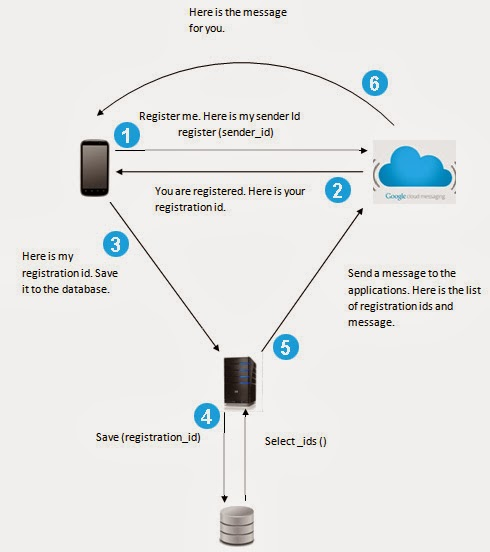
\includegraphics[scale=0.3]{GCM}
\caption{GCM System Architecture}
\label{fig:GCM}
\end{center}
\end{figure}

\section {Key Concepts of GCM}

\subsection {GCM Components}
\begin {enumerate}
  \item\textbf { Client App} – It is a GCM-enabled Android application running on a device. This must be 2.2+ Android OS device with Google Play Store installed, and it must have at least one logged in Google account if the device is running a version lower than Android 4.0.4.

   \item\textbf { 3rd party Application Server }– An application server that you write as part of implementing GCM. The 3rd-party application server sends data via the GCM connection server to Android application on the device.

    \item\textbf {GCM Connection Server} – These are Google-provided servers involved in taking messages from the 3rd-party application server and sending them to the device.

\end {enumerate}

\subsection {GCM Credentials}
\begin {enumerate}
  \item\textbf {Sender ID} – The sender ID is used in the registration process to identify a 3rd-party application server that is permitted to send messages to the device.

    \item\textbf { Application ID} – The Android application that is registering to receive messages.

    \item\textbf { Registration ID } – An ID issued by the GCM servers to the Android application that allows it to receive messages. Once the Android application has the registration ID, it sends it to the 3rd-party application server, which uses it to identify each device that has registered to receive messages for a given Android application.
    
 \item\textbf {    Sender Auth Token} – An API key that is saved on the 3rd-party application server that gives the application server authorized access to Google services. The API key is included in the header of POST requests that send messages.
\end {enumerate}

\section {LifeCycle Flow}
\begin {enumerate}
   \item\textbf {Enable GCM} – Android application running on a mobile device registers to receive messages.
    \item\textbf {Send A Message} – A 3rd-party application server sends messages to the device.
   \item\textbf {Receive A Message} – Android application receives a message from GCM server.
\end {enumerate}

\begin {enumerate}
\item\textbf {Enable GCM}
To use the messaging service on Android application for the first time, it needs to call the GoogleCloudMessaging method register(). The register() method returns a registration ID which should be stored by our Android application for later use.

   \item\textbf { Send A Message} : Here is the sequence of events that occurs when the application server sends a message.
        Message is sent to GCM servers by the application server.
        Google enqueues and stores the message incase the device is offline.
        When the device is online, Google sends the message to the device.
        On the device, the system broadcasts the message to the specified Android application via Intent broadcast with proper permissions, so that only the targeted Android application gets the message. This wakes the Android application up. The Android application does not need to be running beforehand to receive the message.
        The Android application processes the message. If the Android application is doing non-trivial processing, you may want to grab a PowerManager WakeLock and do any processing in a service.

   \item\textbf { Receive A Message} : This is the sequence of events that occurs when an Android application installed on a mobile device receives a message.
        The system receives the incoming message and extracts the raw key/value pairs from the message payload, if any.
        The system passes the key/value pairs to the targeted Android application in a com.google.android.c2dm.intent.RECEIVE Intent as a set of extras.
        The Android application extracts the raw data from the com.google.android.c2dm.intent.RECEIVE Intent by key and processes the data.
\end {enumerate}